
%(BEGIN_QUESTION)
% Copyright 2010, Tony R. Kuphaldt, released under the Creative Commons Attribution License (v 1.0)
% This means you may do almost anything with this work of mine, so long as you give me proper credit

Suppose a technician is troubleshooting this network of digital devices, and suspects an electrical fault somewhere in the network preventing communication.  It seems {\it none} of the devices is able to communicate with any other device on the network:

$$\includegraphics[width=15.5cm]{i02223x01.eps}$$

The technician decides to loosen terminal number 38 and remove the wire entering its left-hand side.  Then, she uses her ohmmeter to measure resistance between terminals 52 and 53.  The ohmmeter registers 152 ohms.

Identify the likelihood of each specified fault for this circuit.  Consider each fault one at a time (i.e. no coincidental faults), determining whether or not each fault could independently account for the ohmmeter measurement as well as the total lack of communication in this network.

% No blank lines allowed between lines of an \halign structure!
% I use comments (%) instead, so that TeX doesn't choke.

$$\vbox{\offinterlineskip
\halign{\strut
\vrule \quad\hfil # \ \hfil & 
\vrule \quad\hfil # \ \hfil & 
\vrule \quad\hfil # \ \hfil \vrule \cr
\noalign{\hrule}
%
% First row
{\bf Fault} & {\bf Possible} & {\bf Impossible} \cr
%
\noalign{\hrule}
%
% Another row
Device {\bf A} failed shorted &  &  \cr
%
\noalign{\hrule}
%
% Another row
Device {\bf B} failed open &  &  \cr
%
\noalign{\hrule}
%
% Another row
Broken wire between terminals 38 and 70 &  &  \cr
%
\noalign{\hrule}
%
% Another row
Right-hand terminating resistor shorted &  &  \cr
%
\noalign{\hrule}
%
% Another row
Device {\bf E} failed shorted &  &  \cr
%
\noalign{\hrule}
%
% Another row
Short between terminals 33 and 34 &  &  \cr
%
\noalign{\hrule}
} % End of \halign 
}$$ % End of \vbox


\vfil

\underbar{file i02223}
\eject
%(END_QUESTION)





%(BEGIN_ANSWER)

This is a graded question -- no answers or hints given!

%(END_ANSWER)





%(BEGIN_NOTES)

The ohmmeter reading of 152 ohms suggests the left-hand terminating resistor is connected, since the cable should exhibit infinite resistance (open) and the devices connected to the cable should likewise exhibit very high impedances.  We also know from the 152 ohm resistance measurement that there are no short-circuits to the left of terminals 38/39.  However, we know nothing about the condition of components to the right of terminals 38/29, and we know that a lack of proper resistive termination or any wiring discontinuities can cause signal reflections sufficient to cripple communication.

% No blank lines allowed between lines of an \halign structure!
% I use comments (%) instead, so that TeX doesn't choke.

$$\vbox{\offinterlineskip
\halign{\strut
\vrule \quad\hfil # \ \hfil & 
\vrule \quad\hfil # \ \hfil & 
\vrule \quad\hfil # \ \hfil \vrule \cr
\noalign{\hrule}
%
% First row
{\bf Fault} & {\bf Possible} & {\bf Impossible} \cr
%
\noalign{\hrule}
%
% Another row
Device {\bf A} failed shorted &  & $\surd$ \cr
%
\noalign{\hrule}
%
% Another row
Device {\bf B} failed open &  & $\surd$ \cr
%
\noalign{\hrule}
%
% Another row
Broken wire between terminals 38 and 70 & $\surd$ & $\surd$ \cr
%
\noalign{\hrule}
%
% Another row
Right-hand terminating resistor shorted & $\surd$ &  \cr
%
\noalign{\hrule}
%
% Another row
Device {\bf E} failed shorted & $\surd$ &  \cr
%
\noalign{\hrule}
%
% Another row
Short between terminals 33 and 34 &  & $\surd$ \cr
%
\noalign{\hrule}
} % End of \halign 
}$$ % End of \vbox


%INDEX% Networking, protocols: CSMA/CD (Ethernet)

%(END_NOTES)


